\section{\uppercase{Best views estimation}}\label{sec:best-views-estimation}

\noindent Estimation of the best views for a constellation of sensors requires both the ability to generate accurate sensor data for each type of sensor and also an efficient approach to compute the surface coverage that we are trying to maximize. The next sections explain how the sensor data is analyzed and also presents the approaches used to estimate the best constellation of sensors for a given simulation world.

\subsection{Reference surface point cloud}

The first step in the processing pipeline includes the generation of the multi-object reference point cloud that is built by transforming the point cloud associated with the target \gls{cad} model into each target object within the simulation world (example shown in \cref{fig:reference-cloud}). Later on, the reference point cloud is filtered with a voxel grid algorithm in order to perform a regular space partition and extract the surface voxels centroids that contain points. This approach allows to generate a reference point cloud with a constant surface point density, which will be critical later on when computing the surface coverage percentage achieved with a given sensor constellation.

\begin{figure}
	\centering
	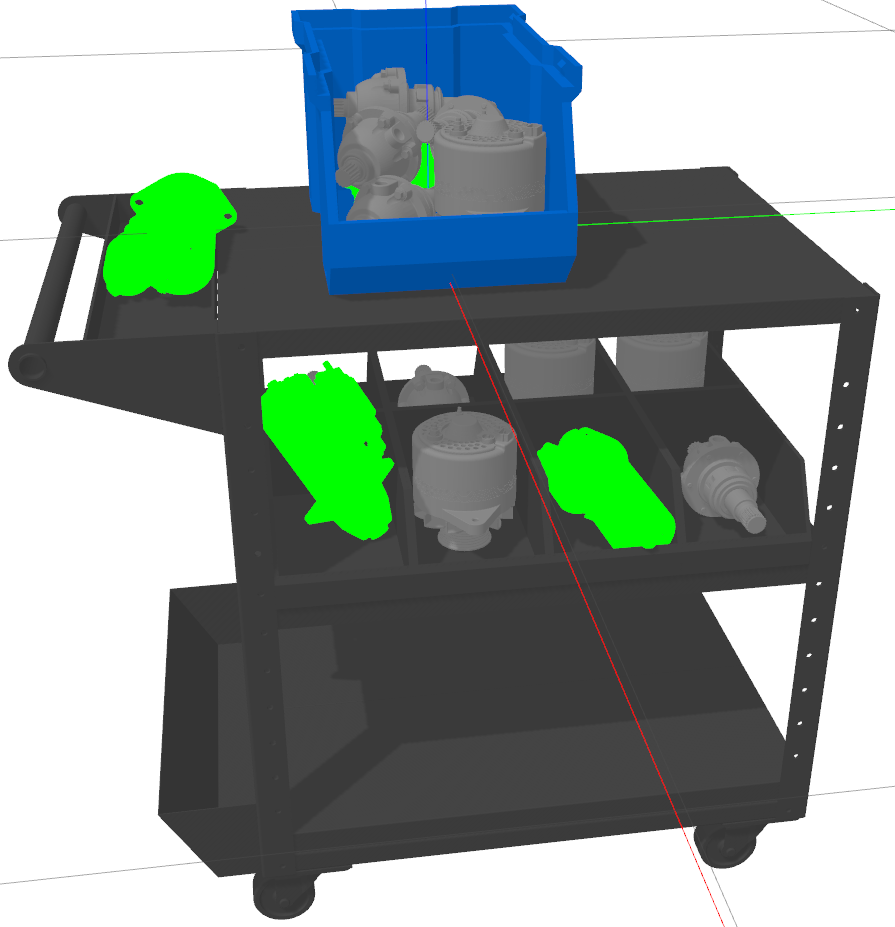
\includegraphics[height=.14\textheight]{sensor-data-processing/multimodel-environment}\hspace{2em}
	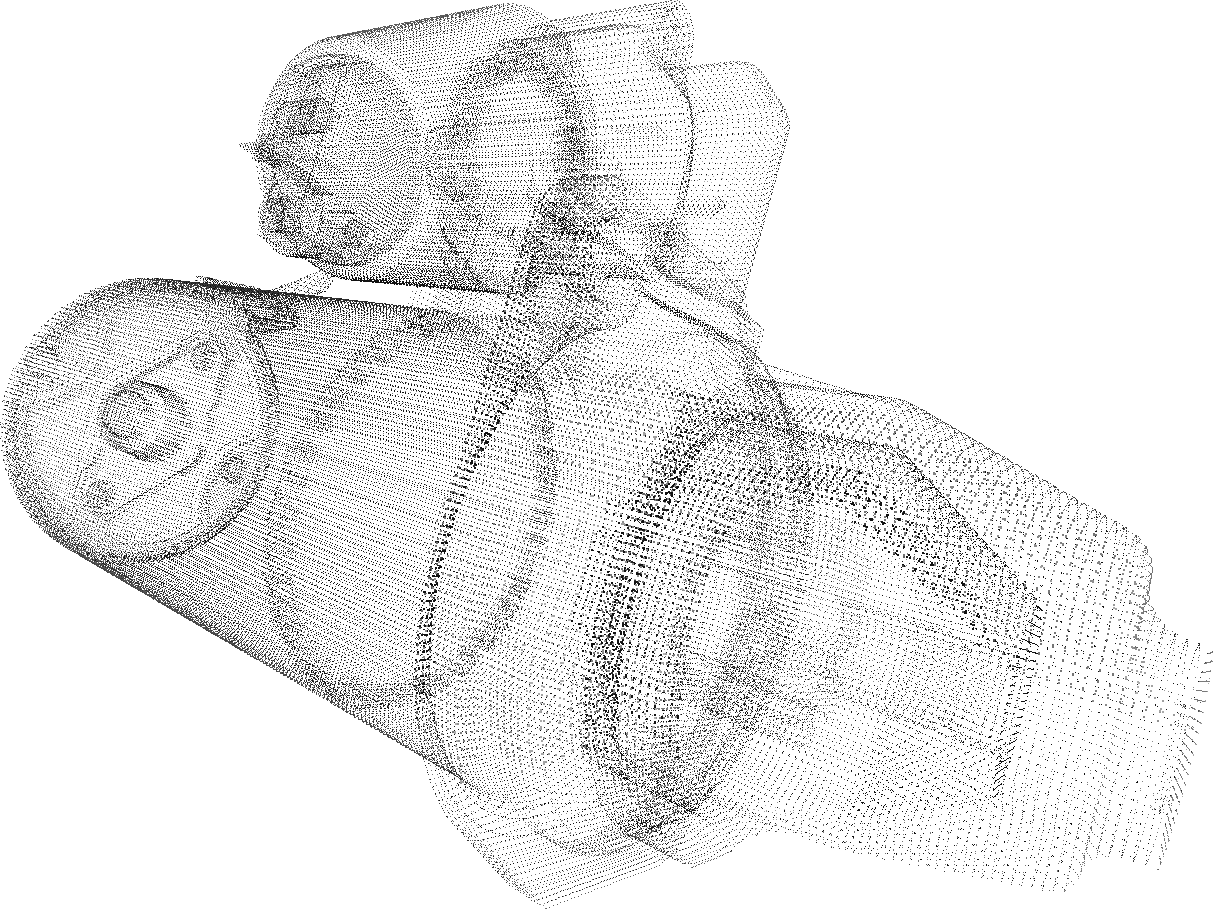
\includegraphics[height=.1\textheight]{sensor-data-processing/cad-model-pointcloud}
	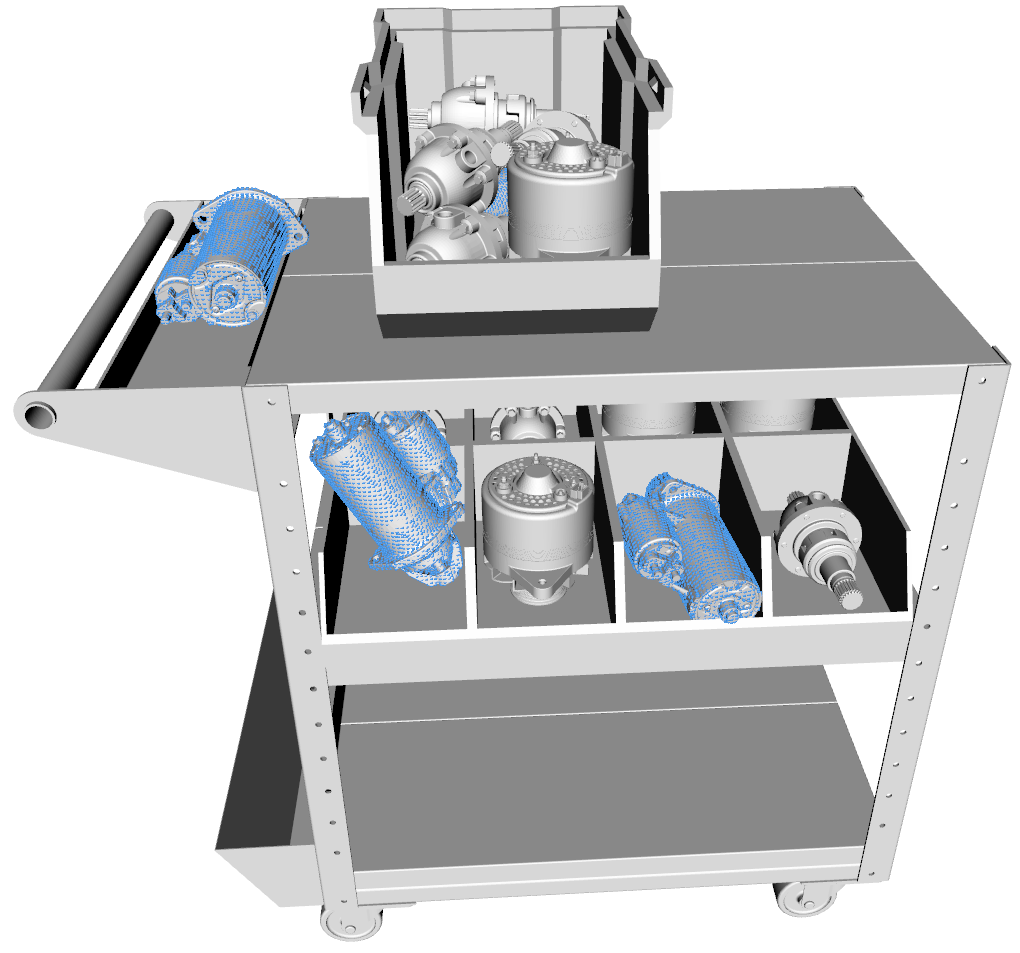
\includegraphics[height=.14\textheight]{sensor-data-processing/multimodel-pointclouds-with-cad}\hspace{2em}
	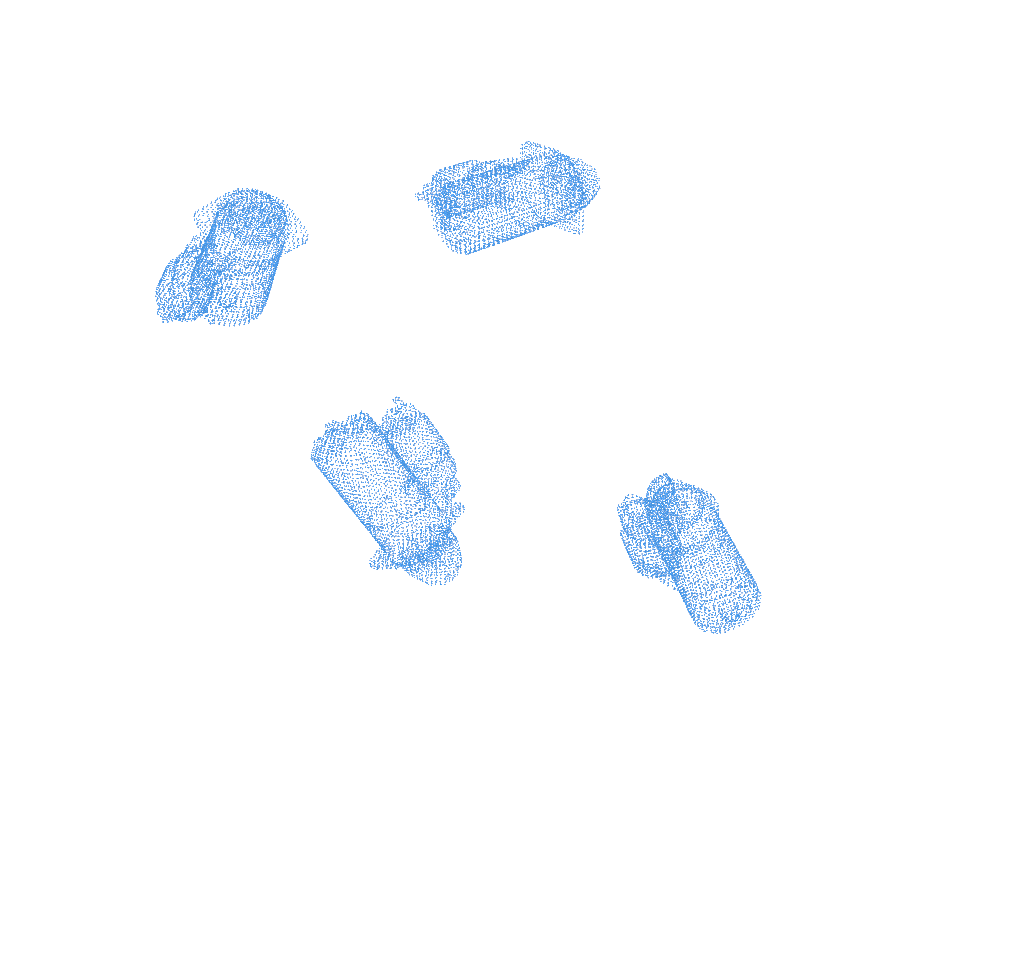
\includegraphics[height=.14\textheight]{sensor-data-processing/multimodel-pointclouds}
	\caption{The first image illustrates the color scene rendering in Gazebo with the target objects in green while the third and fourth images display the reference point cloud that was generated using the CAD point cloud shown on the second image}
	\label{fig:reference-cloud}
\end{figure}


\subsection{Sensors data analysis}

After loading the simulation world 3D models, deploying the sensors populations on the environment and building the filtered reference point cloud, the proposed system generates a color and depth image for every sensor. Then, for each pixel in the color images that have the target objects unique color, the corresponding pixel in the depth image is retrieved and the 3D point is computed using the pinhole model equations shown in \cref{eq:pointcloud}. Later on, the 3D point is transformed from the sensor coordinate system into the world coordinate system (having all sensor data in the same coordinate system allows fast merging of point clouds from several sensors). After processing all pixels of a given image, the associated point cloud is filtered with a voxel grid algorithm in order to perform a regular space partition for extracting the centroid of each voxel containing sensor points. This step is critical for allowing consistent evaluation of the object(s) observed surface area percentage, given that sensors with different resolution or at different distances may generate point clouds with different point density even when observing the same surface area. By performing a point cloud downsampling using a voxel grid algorithm with an appropriate cell size given the geometry we are trying to observe (too many points on a small area do not provide a significant advantage for 3D perception and require more processing time), this problem is mitigated. Moreover, given that that both the reference point cloud and the sensor data point cloud were filtered in the same coordinate frame with the same voxel grid, the surface coverage percentage can be computed very efficiently by simply dividing the number of points in the filtered sensor data point cloud by the number of points in the filtered reference point cloud.

In the end of the sensor analysis stage, each sensor is associated with a filtered point cloud in the world coordinate frame containing only points belonging to the target objects.

\footnotesize
\begin{equation}\label{eq:pointcloud}
	\begin{split}
		X = \frac{(PixelCol - XPrincipalPoint) \times PixelDepth}{XFocalLenght}\\
		Y = \frac{(PixelRow - YPrincipalPoint) \times PixelDepth}{YFocalLenght}\\
		Z = PixelDepth
	\end{split}
\end{equation}
\normalsize

\begin{figure}
	\centering
	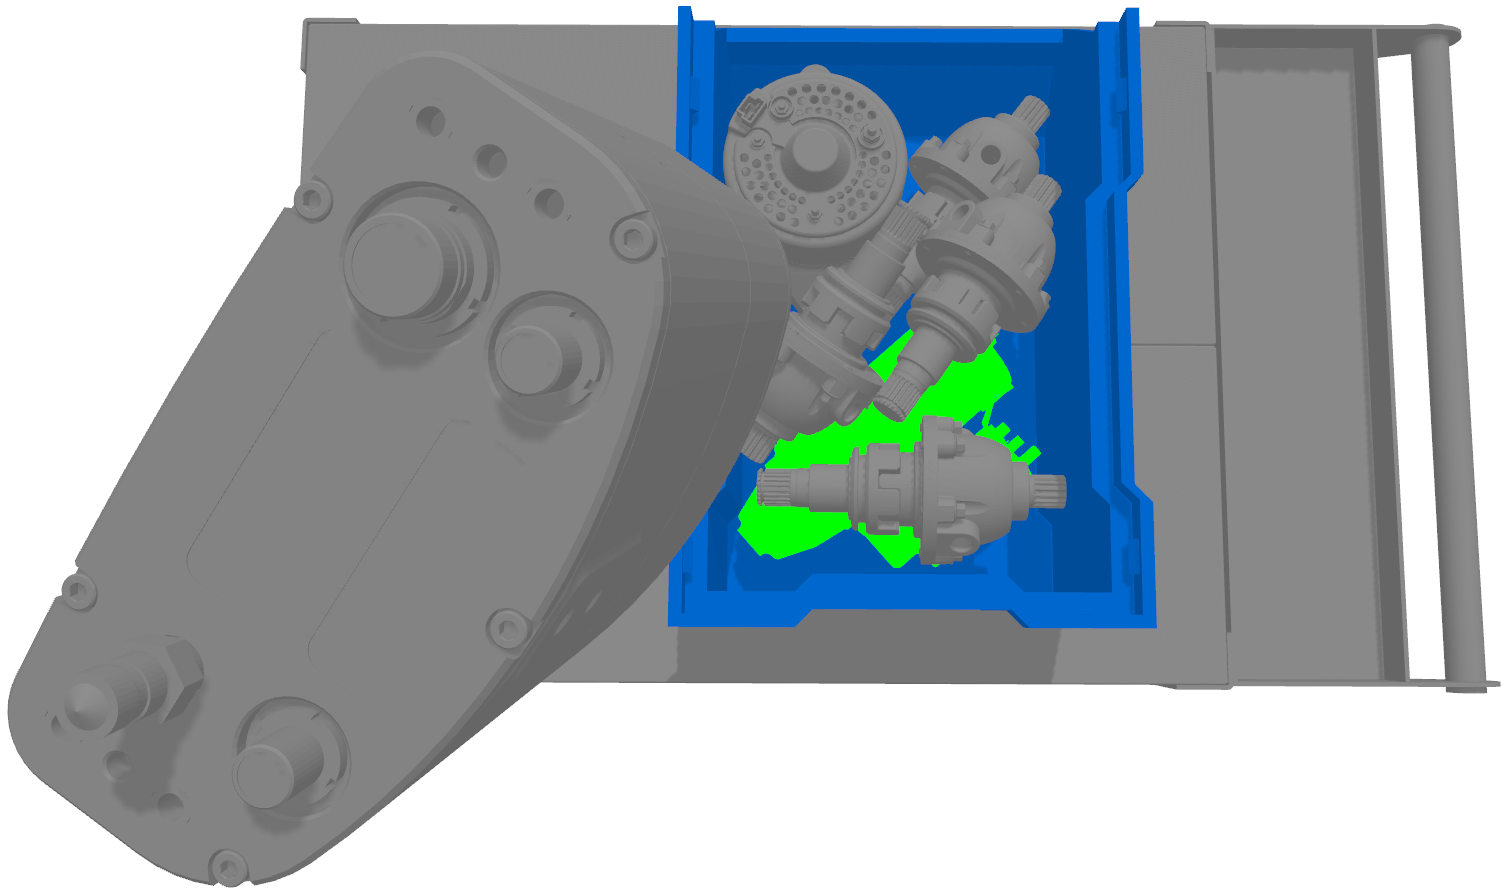
\includegraphics[height=.132\textheight]{sensor-data-processing/sensors-best-view}\\
	\vspace{0.5em}
	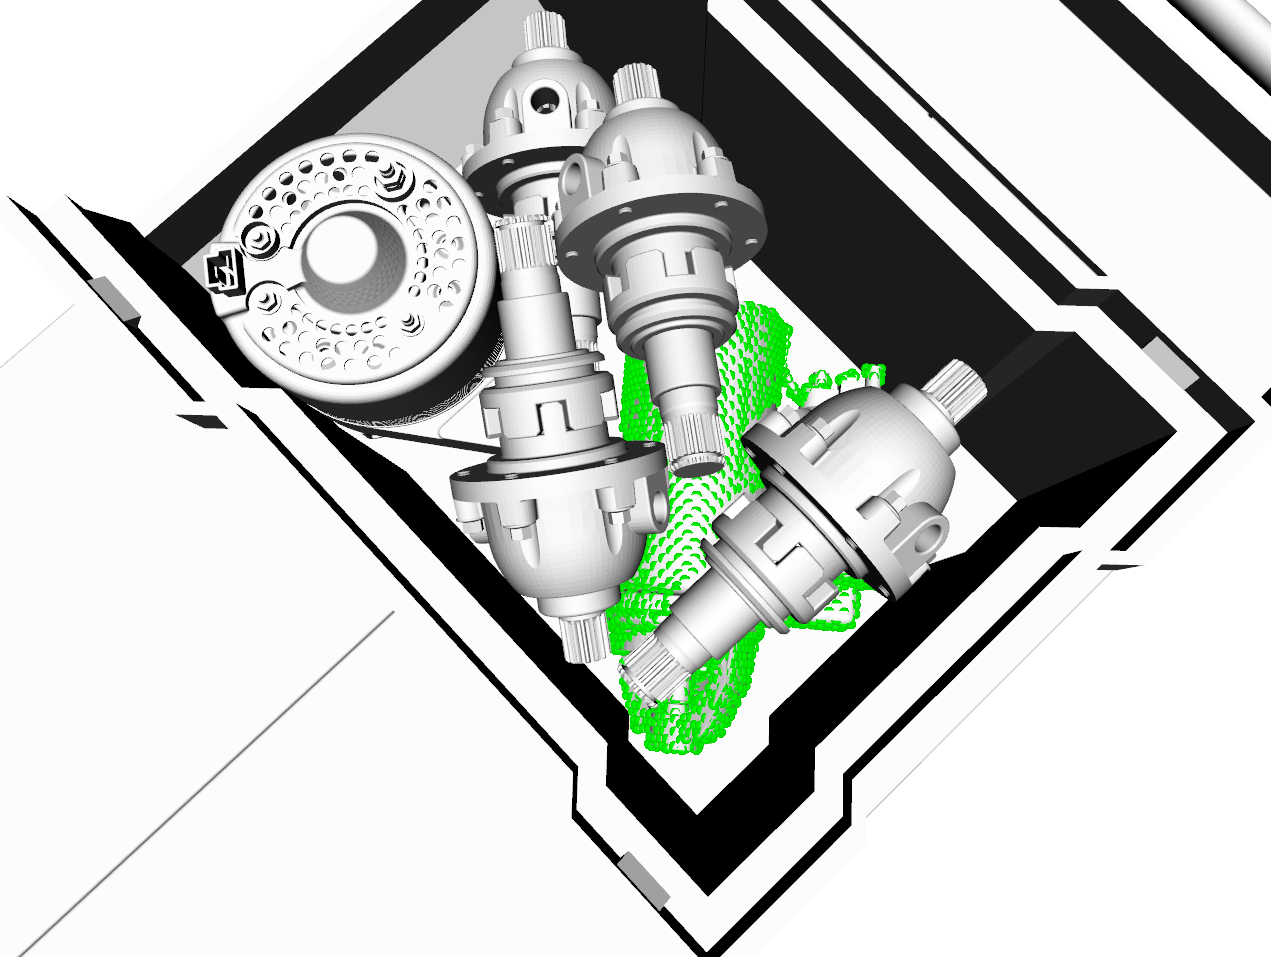
\includegraphics[height=.132\textheight]{sensor-data-processing/rviz-sensor-view}\hspace{2em}
	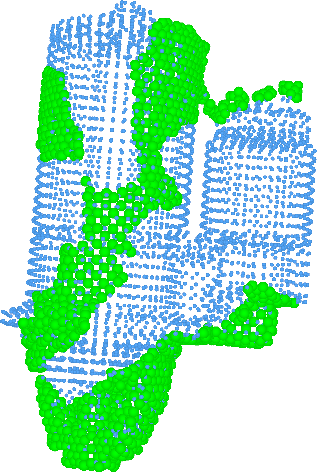
\includegraphics[height=.132\textheight]{sensor-data-processing/rviz-sensor-view-without-cad-with-model}
	\caption{Color image rendered with the Gazebo simulator (top image containing the scene and sensor) along with the generated point cloud for the target object taking into consideration the environment occlusions (bottom images, in which the green spheres are the observed points and the blue spheres are from the filtered point cloud of the associated CAD model)}
\end{figure}


\subsection{Estimation of the best sensor}

After having the processed point cloud for each deployed sensor:
\begin{itemize}
	\item If only one sensor is enough (decision made by the system user):
	\begin{itemize}
		\item The surface coverage percentage for each sensor is computed
		\begin{itemize}
			\item Given that both the reference point cloud and the sensor data were filtered with a voxel grid with the same resolution and in the same coordinate system frame, calculating the surface coverage percentage can be efficiently computed by simply dividing the number of surface voxel points in the sensor data by the number of surface voxel points in the reference point cloud
		\end{itemize}
			\item The sensor that can observe the most surface area percentage of the target object(s) is chosen
	\end{itemize}
\end{itemize}


\subsection{Estimation of the best N sensors disposition}

After having the processed point cloud for each deployed sensor:
\begin{itemize}
	\item If several sensors can be used (decision made by the system user):
	\begin{itemize}
		\item Using a Random Sample Consensus (RANSAC) approach, a set of N sensors is chosen randomly
		\item The sensor data from the selected sensors is merged
		\item The voxel grid filter algorithm is applied to ensure that there is only one point per voxel
		\item The observable surface area percentage for the selected sensors is computed
		\item If the current subset of sensors achieved better observable surface area percentage than the current best, then it becomes the current best views estimation for the sensor disposition
		\item At the end of a given number of iterations or if the observable surface area percentage reaches a given threshold, the search is terminated, returning the best sensor disposition found
	\end{itemize}
\end{itemize}
